
\chapter*{Introduction}
\label{chap:intro}
\addcontentsline{toc}{chapter}{Introduction}


Au sein de l'Union Européenne, 70 $\%$ de la population, soit quasiment 340 millions d'habitants, vivent dans des zones urbaines \cite{europ-commission_data_2017}. 486 villes concentrent, chacune, plus de 100 000 habitants. En France, selon l'INSEE, c'est même plus de 84 $\%$ de la population qui vit dans une zone urbaine, soit plus de 55 millions d'habitants. Cette concentration soulève de grandes questions autour de l'organisation de l'espace urbain afin d'offrir une qualité de vie acceptable aux citadins. En effet, avec de telles densités (environ 3000 habitants/km$^2$ et jusqu'à plus de 21 000  habitants/km$^2$ pour la ville de Paris, la plus dense de l'Union Européenne (UE)), plusieurs formes de pollutions viennent dégrader l'environnement urbain. Des sources de désagrément perçues par le citadin, le bruit est le phénomène qui provoque le plus de gêne après la pollution de l'air. Ce bruit est le fruit des activités humaines, provenant essentiellement du transport qu'il soit routier, ferroviaire ou aérien \cite{zannin_characterization_2013}.
En France, selon un rapport de l'ADEME \cite{europeens2016analyse}, ce sont 52 millions de personnes qui se disent affectées par le bruit et principalement le bruit issu du trafic routier. Plus de 7 millions d'individus sont exposés à des niveaux supérieurs à 65 dB($A$) au quotidien et à plus de 55 dB($A$) la nuit.
Cette exposition quotidienne, à de tels niveaux, n'est pas sans conséquence pour l'être humain. L'impact sur l'organisme humain dû à l'exposition au bruit est observé et étudié depuis de nombreuses années \cite{ising1980health}. Parmi les effets possibles, les plus couramment relevés sont des troubles du sommeil \cite{pirrera2010nocturnal}, de la vigilance et de la concentration, l'augmentation du stress, de la pression artérielle et du rythme cardiaque \cite{babisch2005traffic, babisch2008road}. Cet impact sur la santé a également un coût financier pour la société : en France, ce coût est estimé à plus de 11,5 milliard d'euros par an dont une grande partie (89 $\%$) est imputable au bruit du trafic routier \cite{europeens2016analyse}. De plus, si le bruit en ville impacte la vie des citadins, celui-ci se fait également ressentir auprès de la faune sauvage \cite{dutilleux_anthropogenic_2012, francis2009noise} leur causant également du stress ou en compliquant la communication entre les individus et leur reproduction.\\

À partir de ce constat, il est donc nécessaire et utile de savoir caractériser les environnements sonores urbains (ESU) afin d'estimer les sources sonores présentes, leurs niveaux sonores, leurs répartitions pour ainsi réduire et limiter leurs impacts sur les populations urbaines.
Actuellement les outils les plus répandus pour étudier les ESU se basent sur des modèles prédictifs d'émission sonore et de propagation de 4 sources de bruit : le trafic routier, ferroviaire, aérien et le bruit des Installations Classées pour la Protection de l'Environnement. Ces modèles sont notamment utilisés dans le cas de la cartographie du bruit de trafic imposée par la directive Européenne 2002/49/EC \cite{directive}. Ces cartes de bruit permettent l'estimation des niveaux sonores équivalents pondérés $A$ à travers l'ensemble de grandes villes afin de déterminer les lieux où les niveaux sonores sont élevés (et où des travaux d'aménagement sont réalisables) ou bien ceux préservés par ces sources de bruits. Une des limites principales de ces modèles est la restriction d'informations qu'ils offrent puisque seules les 4 sources de bruit y sont décrites là où l'ESU est un mélange de nombreuses autres sources sonores. De plus, ils ne permettent pas d'appréhender l'ESU à travers la perception qu'en ont les citadins \cite{aumond2017modeling}. 
En conséquence, afin d'avoir une connaissance plus fine et précise des ESU, plusieurs projets s'intéressent actuellement au déploiement de capteurs acoustiques en ville \cite{picaut2017characterization,zambon2017life}. La réalisation de mesures permet de considérer l'ensemble des sources sonores présentes en ville et l'effet de l'architecture de la ville sur la propagation du son. Les applications sont alors diverses : amélioration des cartes de bruits par assimilation des niveaux sonores calculés et mesurés, cartographie des environnements sonores, prise en compte de la perception du citadin, détection d'évènements sonores particuliers \dots{}
La réalisation de mesures nécessite toutefois des outils de traitement du signal adaptés afin de pouvoir caractériser les sources sonores présentes, notamment par l'estimation de leur niveau sonore. Sans cette étape, la prise en compte de l'ensemble des sources sonores, sans distinction, est susceptible de mener à des erreurs d'interprétations. L'étude des contributions des différentes sources sonores, à partir d'enregistrements sonores réalisés dans un environnement urbain, a pour l'instant été peu étudiée. 
La ville est composée de différentes ambiances sonores (parc, quartier résidentiel, boulevard \dots{}) ainsi que de nombreuses sources sonores variées (voiture, oiseaux, bruit de pas et de voix, klaxons, fontaine \dots{}), susceptibles d'être émises simultanément. La formation d'un outil adapté à cette diversité n'est alors pas trivial.


Les travaux de cette thèse ont donc pour objectif de créer un outil permettant de déterminer la contribution du trafic routier en ville en cela qu'il est la source de bruit la plus gênante et que les applications liées à la cartographie de bruit par la mesure sont celles qui, à l'heure actuelle, présente le plus d'intérêt \cite{jagniatinskis2014assessment}. La classe de son \textit{trafic} inclut le bruit de fond routier généré par le flot continu de véhicules et le bruit généré par le passage d'un véhicule émergeant.
Dans le cadre d'enregistrements sonores monophoniques, la tâche est complexe car il faut réussir à déterminer la composante du signal \textit{trafic} à partir d'un seul microphone. Si l'étude de sons environnementaux est de plus en plus traitée via, par exemple, les challenges DCASE \cite{stowell2015detection,mesaros2017dcase} avec la détection de signaux liés au transport ou à la classification de scènes sonores, l'étude et la détermination du niveau sonore de la composante \textit{trafic} parmi des mixtures sonores restent peu étudiées. Récemment, \cite{leiba2017large} réussit à extraire le signal audio du trafic parmi des enregistrements sonores et à suivre la trajectoire du véhicule à partir d'une antenne acoustique composée de 128 microphones et des méthodes d'apprentissages.
Dans le cas de capteurs monophoniques, une approche choisie dans \cite{socoro2017anomalous} consiste à détecter la présence des autres sources sonores pour chaque trame temporelle. Lorsque la source détectée n'est pas reconnue comme \textit{trafic}, celle-ci est rejetée et non considérée dans l'estimation du niveau sonore du trafic routier. Les performances de cet outil sur l'estimation du niveau de bruit du trafic routier sont, pour l'instant, inconnues.
L'approche que nous considérons dans ce travail est différente puisqu'elle implique la méthode de séparation de sources, présentée en Figure \ref{fig:separation_source_intro}. Cette méthode consiste à isoler la contribution d'une seule source parmis une mixture sonore composée de plusieurs sources sonores. Plusieurs applications dans l'audio ont été développées dans le domaine de la musique \cite{smaragdis_non-negative_2003,virtanen_monaural_2007} ou pour de la voix \cite{weninger2012supervised,yilmaz2004blind}. Une fois la source sonore isolée il devient possible d'obtenir de nombreuses informations, et notamment le niveau sonore. Parmi les différentes méthodes existantes, il est nécessaire que celle choisie soit adaptée aux réseaux de capteurs monophoniques et qu'elle prenne facilement en compte le recouvrement temporel des sources sonores. 

\begin{figure}[h]
\centering
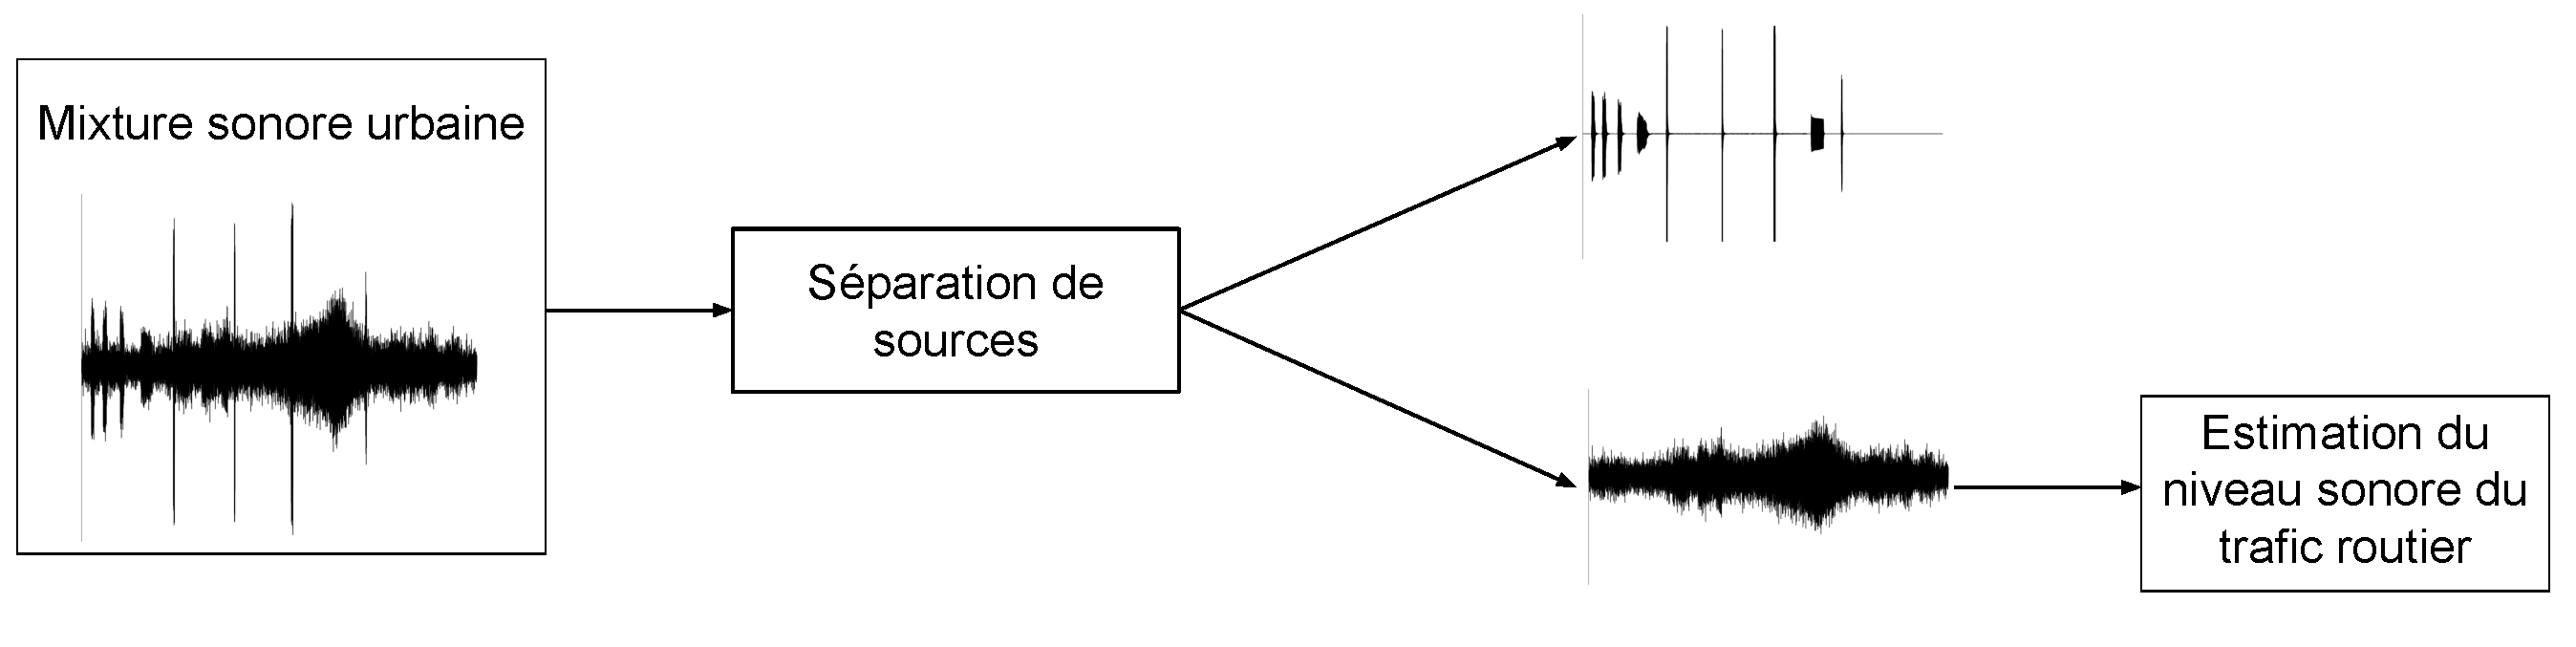
\includegraphics[width=\linewidth]{./figures/autres/schema_source_separation_FR.pdf}
\caption{Schéma de principe de la séparation de sources.}
\label{fig:separation_source_intro}
\end{figure}


En cela, la Factorisation de Matrices Non-négatives (abrégée NMF pour \textit{Non-negative Matrix Factorization} en anglais) \cite{lee_learning_1999} est l'approche retenue dans ces travaux car elle répond bien aux contraintes posées. Là encore, la NMF a été utilisée de très nombreuses fois pour des signaux contenant de la musique \cite{helen2005separation,fevotte_nonnegative_2009} ou de la parole \cite{wilson2008speech,schmidt2006single}. Plusieurs variantes à cette méthode ont été développées dont certaines sont implémentées dans ces travaux. Son application sur une telle source n'ayant jamais encore été réalisée, son fonctionnement nécessite d'être étudié face à de tels environnements sonores. Également, dans le cadre de cette thèse, une nouvelle forme de NMF est proposée, appelée NMF \textit{initialisée seuillé}. 
Afin d'étudier ses performances, la NMF n'est pas appliquée sur des enregistrements audio car l'estimation faite du niveau sonore du trafic ne peut alors pas être comparée à une valeur exacte. En conséquence, elle est appliquée sur des corpus de scènes sonores simulées. L'intérêt de ce procédé est qu'il permet de connaitre les contributions de chacune des sources dont la composante \textit{trafic}. La comparaison du niveau exact et estimé est alors possible.

L'étude de cette thèse consiste donc à mettre en place un protocole expérimental permettant d'estimer le niveau sonore du trafic routier par séparation de source sur des mixtures simulées de scènes sonores urbaines. En cela, plusieurs approches de la NMF sont étudiées afin de définir l'approche optimale obtenant les erreurs d'estimation les plus faibles.

%\section{Plan}

Dans un premier chapitre, la définition formelle de l'objet d'étude, l'ESU, est réalisée. Ensuite, une revue des différentes méthodes visant à le caractériser est réalisée avec un exercice critique de leurs avantages et de leur limites. Au regard des observations faites, une proposition est alors faite décrivant le protocole expérimental mis en place.

Le second chapitre a pour objectif de décrire les différentes méthodes de séparation de sources qui peuvent être envisagées. Ces méthodes sont ensuite comparées selon le cahier des charges défini. La Factorisation en Matrices Non-négatives est alors la méthode retenue. 
Son fonctionnement est présenté en détail dans le chapitre 3 selon les différentes méthodes d'apprentissages ou expressions des fonctions de coût. Ce chapitre introduit également la NMF \textit{initialisée seuillée}, élaborée durant les travaux de ce doctorat. 

Le chapitre 4 est dédié à la réalisation de deux corpus d'évaluation composés de scènes sonores simulés et à la formation d'une base de données permettant de les composer. 
Un premier corpus, nommé \textit{Ambiance}, est construit en mélangeant artificiellement une composante \textit{trafic}, dont le niveau sonore est calibré, avec d'autres classes de sons spécifiques. Ce premier corpus a pour vocation de tester la NMF, d'étudier son fonctionnement et ses performances face à des sons urbains. 
Le second corpus, nommé \textit{SOUR}, est un corpus de scènes sonores réalistes basé sur des enregistrements audio qui ont été réalisés en ville.
L'annotation de ces enregistrements permet de définir une partition temporelle qui sert de base à la construction des scènes sonores. Le rendu obtenu est alors soumis à un test perceptif visant à évaluer le réalisme sonore des scènes simulées. 

Les chapitres 5 et 6 sont ensuite dédiés à l'étude des performances de la NMF soumise aux corpus de scènes sonores. Dans un premier temps, le fonctionnement de la NMF face au corpus \textit{Ambiance} est présenté en détail afin d'étudier le comportement de cette méthode face à de telles mixtures sonores. Les erreurs produites sur l'intégralité du corpus, selon le niveau sonore du trafic et selon chaque classe de son sont présentées. 
Les résultats sur le corpus de scènes sonores réalistes sont ensuite exposés afin d'obtenir la forme optimale de NMF qui pourrait être implémentée dans des capteurs embarqués et utilisée comme outil de traitement du signal \textit{trafic}. Des méthodes d'optimisation sont alors proposées afin d'améliorer les performances de la NMF.